\section{System Features}
\label{sec:system_features}
\writer{Juan}

In this section we will start by presenting a general overview of the software being developed, 
showing its main components and how they will interact with the user, as well as with each other. 
Afterwards, we will go into more detail in order to find out what part each component will play 
during the execution of the program, describing the various functionalities each one will or may provide. 
Specific use cases showing the interaction between each component and the users are also provided, 
showing how they can be used and what is offered to the users.

\begin{figure}[htp]
\begin{center}
  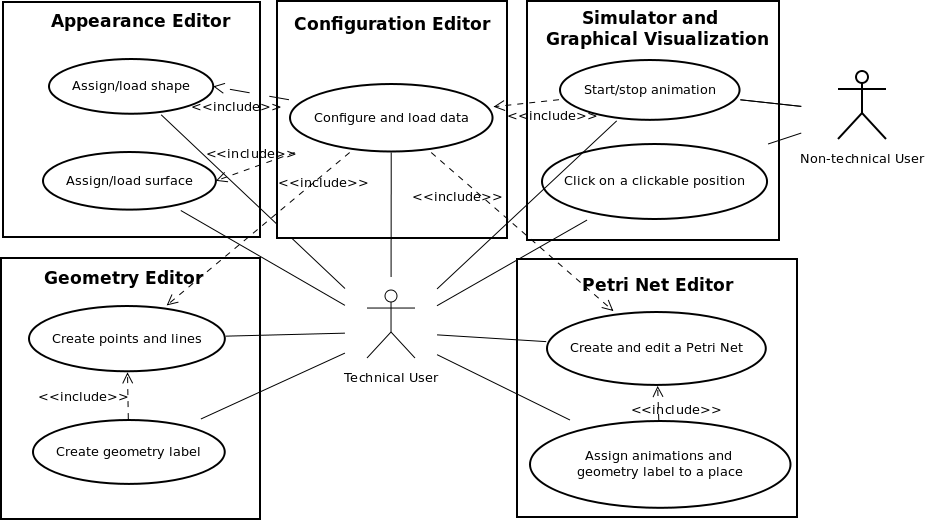
\includegraphics[scale=0.5]{image/uc_general.png}
  \caption{System Use Cases}
  \label{fig:system_use_cases}
\end{center}
\end{figure}

In Figure~\ref{fig:system_use_cases} we can see the manner in which the different components of the software in
development interact with each other and in what way they use one another. External to the software are 
the technical and non-technical user, who are given a set of functionalities to work with. As we can see, 
the technical user will be making use of the editors to set up everything that is needed for the Petri net simulation/visualization. He/She (or any 
non-technical user) will then be able to view the simulation thanks to the Simulator and Graphical 
Visualization component.

\subsection{Petri net Editor}
\index{Petri net!Editor}
\writer{Pablo}

This component will extend the ePNK tool to provide new features to the user, 
such as Input Places. It will also include the Animation Editor, which provides the user with a way of 
creating and configurating the animations for the Petri net that will be simulated. The user will be able 
to assign different Animations to be executed when Tokens reach different Places of the Petri net with this functionality.

\subsubsection{Functional requirements}

\begin{enumerate}
  \item The Petri net editor \textbf{shall} allow the user to create and edit Places.
  \item The Petri net editor \textbf{shall} allow the user to create and edit Transitions.
  \item The Petri net editor \textbf{shall} allow the user to create and edit Arcs to connect Places and Transitions.
  \item The Petri net editor \textbf{shall} allow the user to create and edit Tokens inside Places.
  \item The Petri net editor \textbf{shall} allow the user to create and edit Input Places.
  \item The Petri net editor \textbf{shall} allow the user to assign and edit Labels to the objects created.
  \item The Petri net editor \textbf{shall} allow the user to assign Animations to Places of the Petri net.
  \item The Petri net editor \textbf{shall} create a Petri net and Animation Configuration file that can be read by the Simulator.
  \item The Petri net editor \textbf{shall} allow the user to define a Sequence of Animations.
  \item The Petri net editor \textbf{shall} establish a relationship between a defined Geometry and a Place in the Petri net.
  \item The Petri net editor \textbf{shall} allow the user to save Petri net models.
  \item The Petri net editor \textbf{shall} allow the user to load existing models.
  \item It \textbf{would be nice} to allow the user to save a Sequence of Animations specifying a name for it to use it whenever he or she wants.
  \item It \textbf{would be nice} to give the user a preview of a defined Animation.
\end{enumerate}

\subsubsection{Use Cases}
\index{Petri net!Use cases}
See Figure~\ref{fig:petrinet_use_cases} for the Petri net Editor's use cases. The main features of this editor are shown, specifying the
functionalities provided by our system to allow 3D visualization.

\begin{figure}[htp]
\begin{center}
  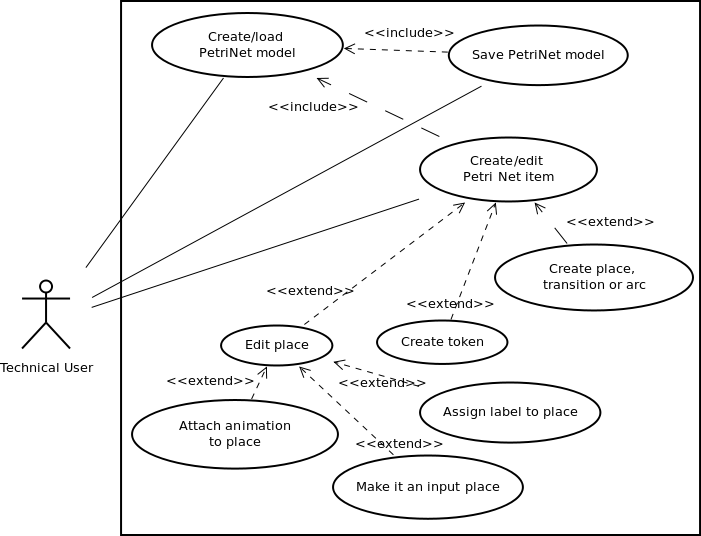
\includegraphics[scale=0.5]{image/uc_petrinet.png}
  \caption{Petri net Use Cases}
  \label{fig:petrinet_use_cases}
\end{center}
\end{figure}

\subsection{Geometry editor}
\index{Geometry!Editor}
\writer{Juan}

This component allows users to create a Geometry for the designed Petri net. It will allow him/her to define a 
Geometry for the Places of said Petri net.

\subsubsection{Functional requirements}

\begin{enumerate}
  \item The Geometry Editor \textbf{shall} allow the user to create points.
  \item The Geometry Editor \textbf{shall} allow the user to create lines connecting two points.    
  \item The Geometry Editor \textbf{shall} create a Geometry Configuration file that can be read by the configurator.
  \item The Geometry Editor \textbf{shall} allow the user to establish a relationship between a Geometry item and 
  its Appearance from the Appearance Configuration.
  \item The Geometry Editor \textbf{should} allow the user to create curves defined by a limited number of intermediate points.
  \item The Geometry Editor \textbf{shall} allow the user to load a Geometry Configuration.
  \item The Geometry Editor \textbf{shall} allow the user to save a Geometry Configuration.
  \item It \textbf{would be nice} to allow the user to create curves defined by any number of intermediate points.
  \item It \textbf{would be nice} to provide a history of the previous actions performed during the current editing process (for Redos, Undos...).
  \item It \textbf{would be nice} to provide the user a set of predefined figures like circunferences or squares.
  \item It \textbf{would be nice} to allow the user to save figures.
  \item It \textbf{would be nice} to allow the user to assign different lengths to the figures added in order to represent real proportions.
\end{enumerate}

\subsubsection{Use Cases}
\index{Geometry!Use cases}

See Figure~\ref{fig:geometry_use_cases} for the Geometry Editor's use cases.

\begin{figure}[htp]
\begin{center}
  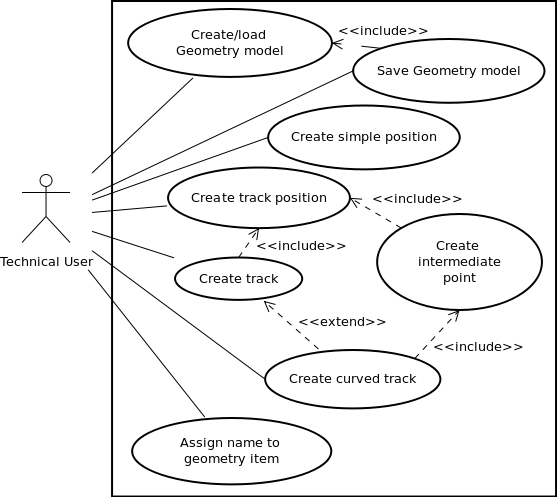
\includegraphics[scale=0.5]{image/uc_geometry.png}
  \caption{Geometry Use Cases}
  \label{fig:geometry_use_cases}
\end{center}
\end{figure}

\subsection{Appearance editor}
\index{Appearance editor}
\writer{Juan}

This component allows the user to set the shape and surface of the objects
belonging to the visual representation of the Petri net to be simulated.

\subsubsection{Functional requirements}

\begin{enumerate}
  \item The Appearance Editor \textbf{shall} allow the user to create 3D objects by choosing a predefined simple shape.
  \item The Appearance Editor \textbf{shall} allow the user to create surfaces by choosing a predefined color.
  \item The Appearance Editor \textbf{shall} create an Appearance Configuration file that can be read by the Configurator.
  \item The Appearance Editor \textbf{shall} allow the user load an Appearance Configuration.
  \item The Appearance Editor \textbf{shall} allow the user to save an Appearance Configuration.
  \item The Appearance Editor \textbf{should} allow the user to create 3D objects by referencing an existing 3D model.
  \item The Appearance Editor \textbf{should} allow the user to create surfaces by referencing an existing texture.
  \item The Appearance Editor \textbf{should} allow the user to assign a surface to a 3D object.
  \item It \textbf{would be nice} to provide the user with a collection of pre-defined complex shapes.
  \item It \textbf{would be nice} to allow the user to choose the colour from a palette.
\end{enumerate}

\subsubsection{Use Cases}
\index{Appearance editor!Use cases}

See Figure~\ref{fig:appearance_use_cases} for the Appearance Editor's use cases.

\begin{figure}[htp]
\begin{center}
  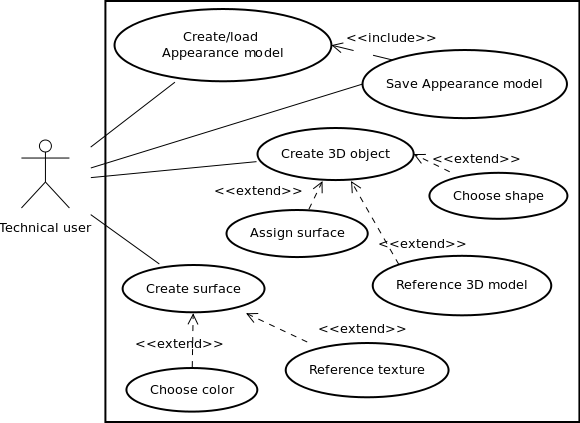
\includegraphics[scale=0.5]{image/uc_appearance.png}
  \caption{Appearance Use Cases}
  \label{fig:appearance_use_cases}
\end{center}
\end{figure}

\subsection{Configuration Editor}
\index{Configuration editor}
\writer{Juan}

This component allows the user to configure a simulation, by connecting the Petri
Net, Geometry and Appearance files used in the simulation and visualization.

\subsubsection{Functional requirements}

\begin{enumerate}
  \item The Configuration Editor \textbf{shall} allow the user to set a reference to the file containing the Petri net and Animations Configuration.
  \item The Configuration Editor \textbf{shall} allow the user to set a reference to the file containing the Geometry.
  \item The Configuration Editor \textbf{shall} allow the user to set a reference to the file containing the Appearance.
  \item The Configuration Editor \textbf{shall} allow the user to start the visualization of the simulation with the configured data.
  \item It \textbf{would be nice} to allow the user to set some aditional attributes that are not related to a concrete editor 
  (e.g. default track width or background color).
  \item It \textbf{would be nice} if, once the Petri net is loaded, the Geometry and Appearance Configurations are detected automatically based on name and extension.
\end{enumerate}

\subsubsection{Use Cases}
\index{Configuration editor!Use Cases}

See Figure~\ref{fig:configuration_use_cases} for the Configuration Editor's use cases.

\begin{figure}[htp]
\begin{center}
  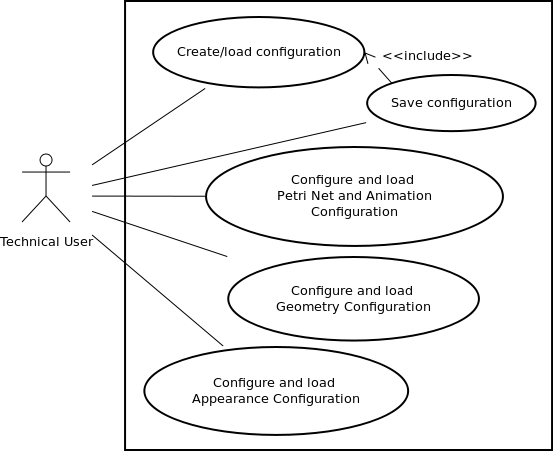
\includegraphics[scale=0.5]{image/uc_configurator.png}
  \caption{Configuration Use Cases}
  \label{fig:configuration_use_cases}
\end{center}
\end{figure}

\newpage
\subsection{Simulation and Graphical visualization tool}
\writer{María}

This component simulates the behaviour of the Petri net and provides a 3D
visualization of the objects defined for it, as well as the corresponding animations.

\subsubsection{Functional requirements}

\begin{enumerate}
  \item The graphical visualization functionality \textbf{shall} show a 3D visualization of the Geometry defined in the Geometry Configuration.
  \item The graphical visualization functionality \textbf{shall} show a 3D visualization of the Animations.
  \item The graphical visualization functionality \textbf{shall} detect when a user interacts with the visualization, i.e. clicks on a clickable position.
  \item The graphical visualization functionality \textbf{shall} allow the user to start/stop the animation.
  \item The graphical visualization functionality \textbf{should} allow the user to pause/restart the animation.
  \item The simulation functionality \textbf{shall} simulate the given Petri net.
  \item The simulation functionality \textbf{shall} allow the user to start as many simulations of the same Petri net as he or she wants.  
  \item It \textbf{would be nice} to load a Petri net at initialization and allow the user to edit it in parallel without interfering with the simulation.
  \item It \textbf{would be nice} to offer a visualization of the changes in the Petri net during the simulation.
\end{enumerate}

\subsubsection{Use Cases}

See Figure~\ref{fig:simulation_use_cases} for the Simulation \& Graphical Visualization tool's use cases.

\begin{figure}[htp]
\begin{center}
  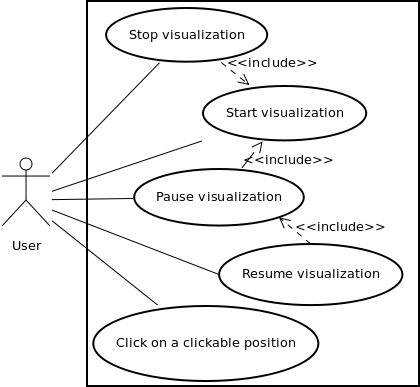
\includegraphics[scale=0.5]{image/uc_visualization.png}
  \caption{Simulation and Graphical Visualization Use Cases}
  \label{fig:simulation_use_cases}
\end{center}
\end{figure}


